\subsection{Skalarum}
En Detektor skal være robust overfor små geometriske og fotometriske deformationer samt støj. Geometriske forskelle kan omfatte rotation, skalering og ændring af perspektiv.  Fotometriske forskelle kan omfatte ændringer i belysning (f.eks. ved delvist overskyet vejr) eller forskelle i refleksion mod de to drone-positioner hvorfra billederne er optaget. En god detektor skal være invariant eller robust over for sådanne forskelle.  Flere artikler understreger nødvendigheden for skalainvarians hos detektorer og at problemet skal konfronteres i alle billedbehandlings situationer \cite{koen} \cite{blob} \cite{lindenscale}. Denne sektion beskriver, hvordan en sådan invarians kan opnås. \\ \\
Objekter i virkeligheden, såvel som detaljer i et billede, optræder kun som meningsfulde enheder over et specifikt skalainterval. Et træ vil indenfor centimeters eller nanometers afstand optræde som blade eller molekyler og indenfor meters afstand som et træ. Koenderink \cite{koen} definere et objekts skalainterval som værende afgrænset af to skalaer: den inderste og den yderste skala,  F.eks. vil en trætop have en indre skala på ca. 10 cm og en ydre skala på ca. 10 m. Da billedet indeholder en ukendt scene, vides det ikke hvilket skalainterval, der for et givent objekt indgående i scenen, er meningsfuldt. Den inderste skala af billedet vil derfor være bundet af pixelstørrelsen og den ydre af billedets fysiske størrelse. En aksiomatisk tilgang til det ukendte skalainterval er at undersøge en bred skalarepræsentation af billedet i form af en udvidelse af billedfunktionen med en enkelt parameter også kaldt skalaparametren $\sigma$:
\begin{equation}
\begin{split}
&L: R^3 \rightarrow R \\
&L(x,y,\sigma) = \lambda \hspace{0.5 cm} (x,y,\sigma)\in R^3, \lambda \in R
\end{split}
\end{equation}
For at opnå en multi-skala repræsentation af billedet, oprettes der et skalarum bestående af skalabilleder, der går fra at udtrykke finere til grovere strukturer, proportionelt med skalaparametren, som illustreret i figur \ref{fig:scalerep}. 
\begin{figure}[H]
    \centering
    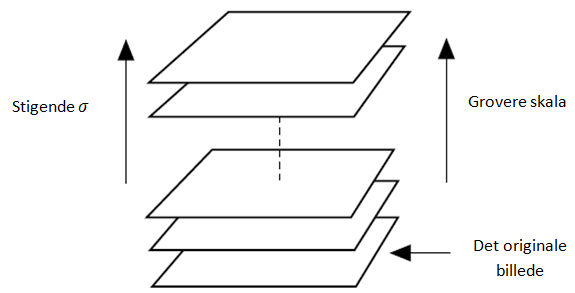
\includegraphics[width=0.55\textwidth]{fig/32.png}
     \vspace{-1em}
    \begin{center}    
       \caption{\textcolor{gray}{\footnotesize \textit{ }}}
    \label{fig:scalerep}
     \end{center}
     \vspace{-2.5em}
  \end{figure} \noindent
Denne overgang fra finere til grovere strukturer kan opnås ved iterativt at folde billederne med et Gaussisk filter af stigende $\sigma$ værdi, hvor billedets nulskala repræsenteres ved biledet $ L(x,y,0) = I(x,y)$ og for $\sigma>0$:
\begin{equation}
L(x,y,\sigma) = G(x,y,\sigma)\ast I(x,y)
\label{scalespace1}
\end{equation}
\\
Der anvendes et Gaussisk filter, på grund af dens unikke egenskaber,  bl.a. at der ikke forekommer nye strukturer ved glatning, når skalaparametren stiger. Glatningen af billedet kan ses som at billedet flades ud og derved vil intensiteten i maksima falde og stige i minima.  Witkins \cite{witkins} beviste dette i tilfældet for én-dimensionselle signaler illustreret i  figur  \ref{scalespace1}, der viser resultatet af at glatte et signal med et Gaussisk filter af stigende $\sigma$ værdi. Det ses tydeligt, hvordan signalets underliggende grovere struktur bliver udtrykt og at finere strukturer undertrykkes.
\begin{figure}[H]
    \centering
    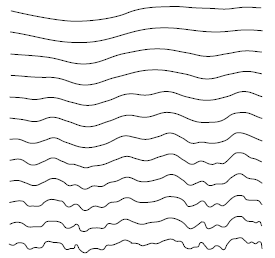
\includegraphics[width=0.45\textwidth]{fig/33.png}
     \vspace{-1em}
    \begin{center}    
       \caption{\textcolor{gray}{\footnotesize \textit{Et én-dimensionalt signal udsat for et Gaussisk filter af gradvist stigende størrelse.}}}
    \label{fig:scalereps}
     \end{center}
     \vspace{-2.5em}
  \end{figure} \noindent
Koenderink \cite{koen} førte dette begreb videre til det to-dimensionelle tilfælde, ved at vise at foldningen af billedet med et Gaussisk filter er den generelle løsning til diffusionsligningen, som beskriver hvordan en varmefordeling $I$ udvikler sig over tid $t$.
$$ \partial t I = \nabla^2I $$
dvs. varmefordelingen kan for et givent tidspunkt udledes ved at folde den originale fordeling med et Gaussisk filter, hvor størrelsen er direkte relateret til tiden for varmefordelingen. Beskriver figur \ref{fig:scalereps}, en varme udvikling over en tid, hvor forskellige udviklinger er illustreret, vil alle dens udviklinger fra starttilstanden være dens skalarum.
\subsubsection*{Skala Pyramide}
En udbredt metode, hvorpå skalarummet kan repræsenteres, er ved en \textit{skalapyramide}. Ved en skalapyramide repræsentation oprettes en pyramide af kopier af det undersøgte billede, der for hvert niveau i pyramiden reduceres i størrelsen af billedet. For at undgå uægte strukturer, der kan opstå som resultat af ændring i billedets opløsning, anvendes der imellem hvert niveau af pyramiden et Gaussisk filter, inden billederne reduceres. \begin{figure}[H]
    \centering
    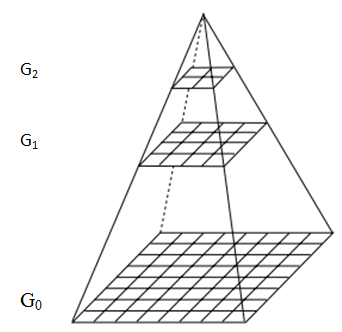
\includegraphics[width=0.40\textwidth]{fig/40.png}
     \vspace{-1em}
    \begin{center}    
       \caption{\textcolor{gray}{\footnotesize \textit{ }}}
    \label{fig:scalerepdiff}
     \end{center}
     \vspace{-2.5em}
  \end{figure} \noindent
Hvis $G_0$ er det originale billede, der repræsenteres i skalapyramiden, kan de forskellige niveauer opnås ved:
\begin{equation}
G_l(i,j)=\sum\limits_{m}\sum\limits_{n}w(m,n)G_{l-1}(2i+m,2j+n)
\end{equation}
hvor $w$ er et Gaussisk filter. Fordelene ved en pyramide repræsentation er at billedernes størrelser reduceres, hvilket reducere antallet af beregninger drastisk. \\
For et billede af en trætop, taget med forskellige afstande, vil en bred skalarepræsentation af billedet sikre at trætoppen vil kunne identificeres til at være ens.
%Måske noget konkluderende til sidst om hvordan dette hjælper på skalainvarians